\documentclass[a4paper, 10pt]{article}
\usepackage[margin = 1in]{geometry}
\usepackage{amsmath}
\usepackage{tabularx}
\usepackage{framed}
\setlength{\parindent}{0em}
\newcolumntype{L}{>{\arraybackslash}m{10cm}}
\newcolumntype{T}{>{\arraybackslash}m{6cm}}
\usepackage{graphicx}
\usepackage{pdfpages}

\begin{document}

\section*{Topic 17 - Electromagnetic Induction}

\section{Faraday's law of electromagnetic induction}

\begin{framed}
   \textbf{Faraday's law of electromagnetic induction} states that the induced e.m.f. is proportional to the rate of change of magnetic flux linkage

   \[
      \text{induced e.m.f.} = -\frac{d \Phi}{dt} 
   \]
   where $\Phi$ is the \textbf{magnetic flux linkage}
\end{framed}	

\section{Magnetic flux and magnetic flux linkage}

\subsection{Magnetic flux}

\begin{framed}
   \textbf{Magnetic flux, $\phi$ }is defined as the product of an area and the component of the magnetic flux density perpendicular to that area \\

   For an area $A$ where a uniform magnetic field with magnetic flux density $B$ passes at an angle $\theta$ 
   \begin{center}
      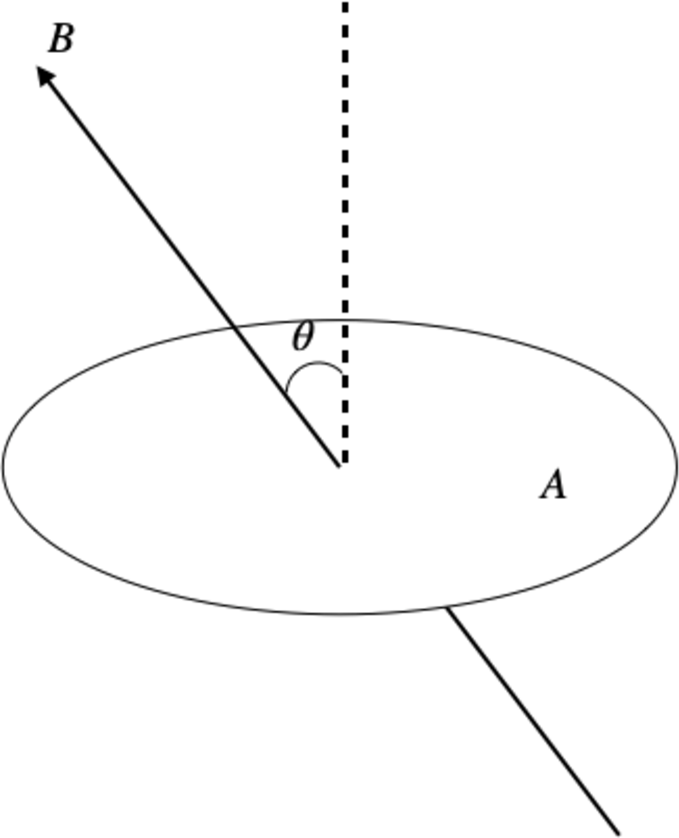
\includegraphics[width=3cm]{figures/1.pdf} 
   \end{center}	

   \[
      \phi = BA cos \theta
   \]
   
\end{framed}	

\subsection{Magnetic flux linkage}
\begin{framed}
   The \textbf{magnetic flux linkage, $\Phi$ } of a coil is the product of the magnetic flux through the voil and the numebr of turns of the coil \\

   For a coil of $N$ turns with uniform cross sectional area $A$ 
   \[
   \Phi = N \phi
   \]
\end{framed}


\section{Determining direction of induced current}
\textbf{NOTE}: there will only be an induced current if there is an induced e.m.f. and \textbf{the circuit is closed}

\subsection{Fleming's right hand rule}
\begin{center}
DO NOTE QUOTE OFR ANSWERING QUESTIONS
\end{center}	

\begin{center}
   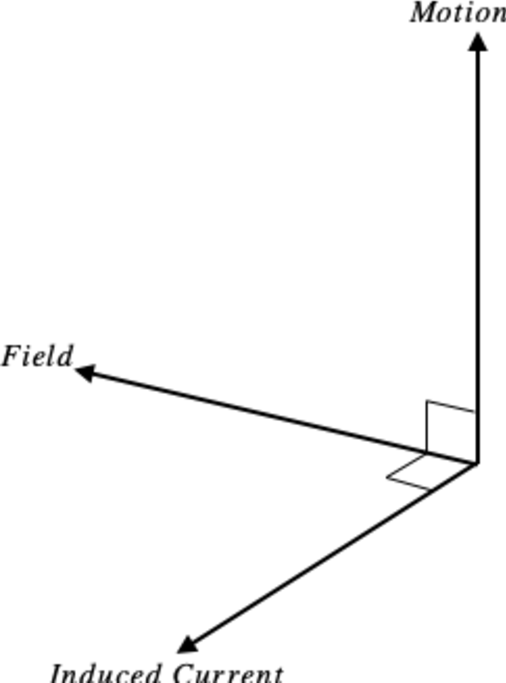
\includegraphics[width=3cm]{figures/2.pdf} 
\end{center}	


\subsection{Lenz's law}

\begin{framed}
   \textbf{Lenz's law} states that the direction of induced e.m.f. is such as to cause effects to oppose the change producing it
\end{framed}	
\begin{itemize}
   \item a result of conservation of energy
\end{itemize}	


\subsection{By first principles}

\begin{itemize}
   \item consider movement of free electrons inside a conductor
   \item consider direction of conventional current due to movement of conductor and hence electrons
   \item determine force on free electrons due to \textbf{Fleming's left hand rule}
   \item electrons will tend towards one end, while positive charge tends towards the other
   \item the separation of cahrge sets up an electric field. 
\end{itemize}	

\begin{framed}
   NOTE THAT 
   \begin{itemize}
      \item outside an e.m.f. source, current flows from \textbf{high to low} potential
      \item inside an e.m.f. source, current flows from \textbf{low to high} potential
   \end{itemize}	
\end{framed}	

\section{Metal rod moving across uniform magnetic field}

\begin{center}
   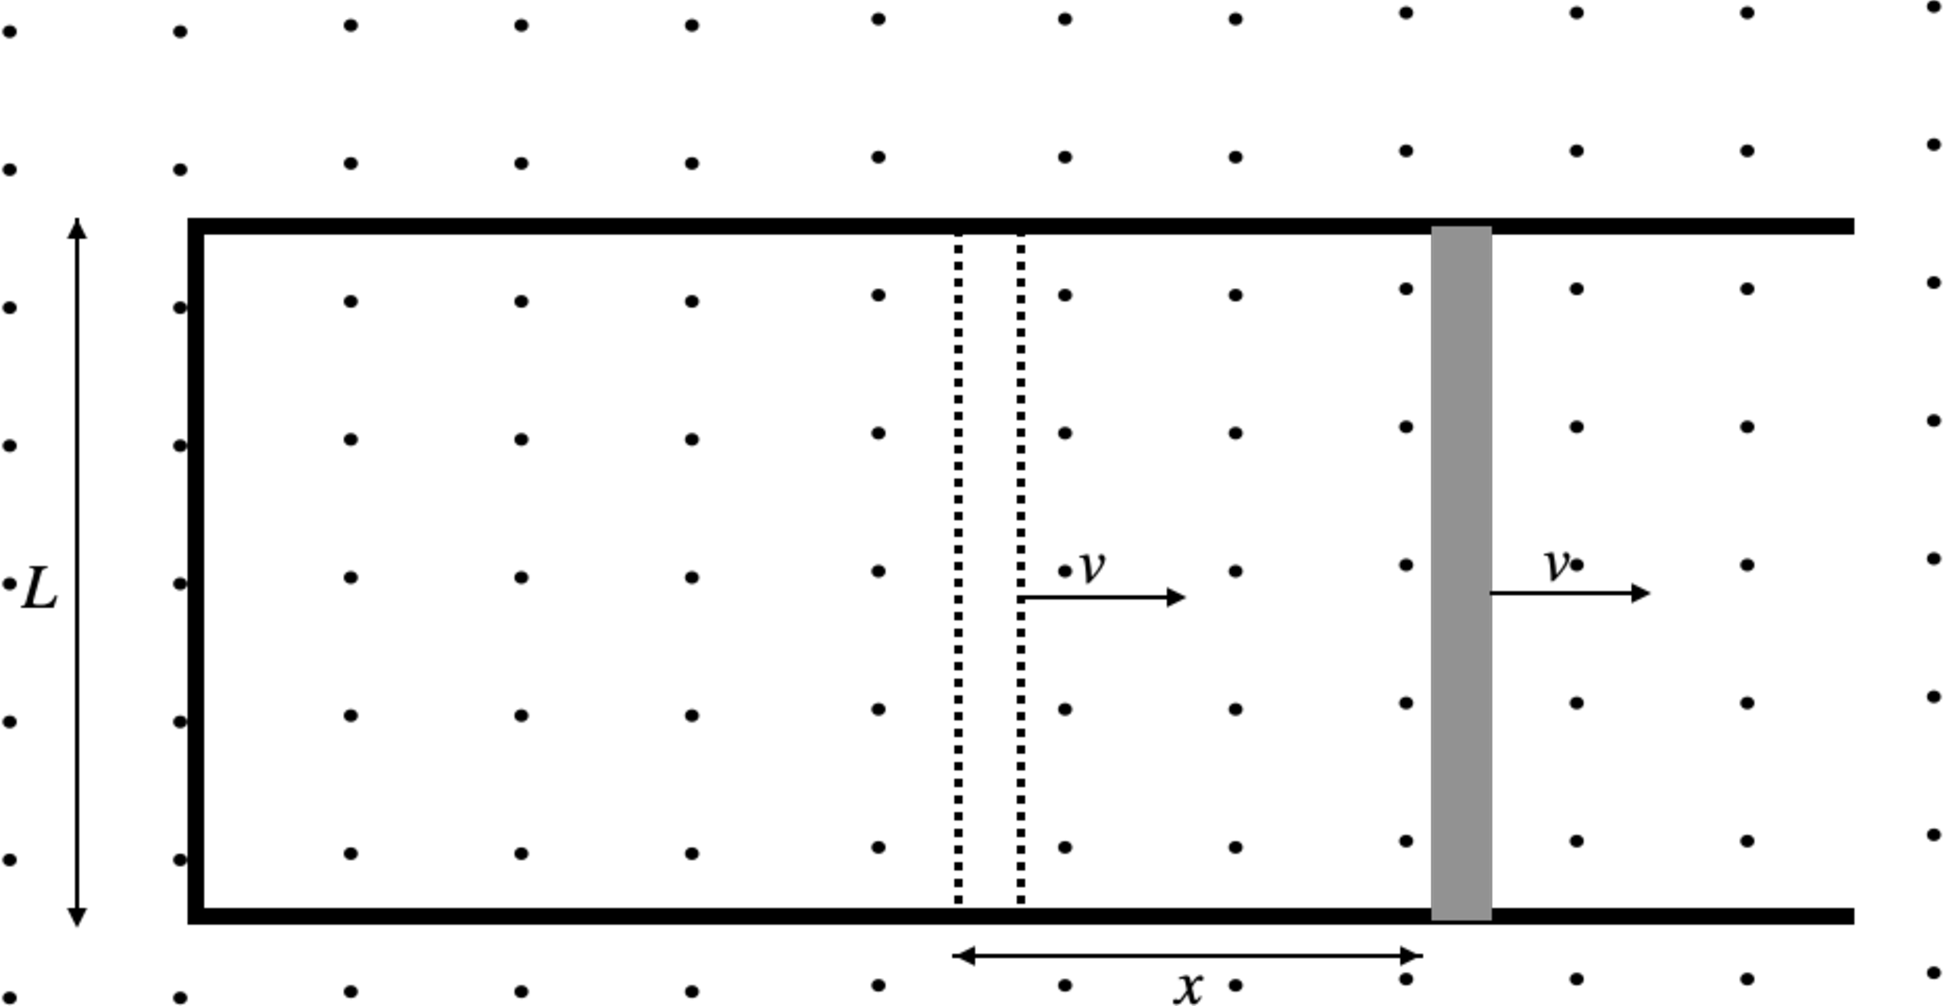
\includegraphics[width=3in]{figures/3.pdf} 
\end{center}	
\begin{itemize}
   \item the distance travelled by rod in time $t$ is $x$
   \item the magnetic flux linkage in time $t$ is 
      \[
      \Phi = BA = BLx
      \]
   \item The magnitude of induced e.m.f. is given by Faraday's law
      \[
      |E| = \left| - \frac{d\Phi}{dt}\right| = BL \frac{dx}{dt} = BLv
      \]
\end{itemize}	

\section{Rotating disc in uniform magnetic field}
\begin{center}
   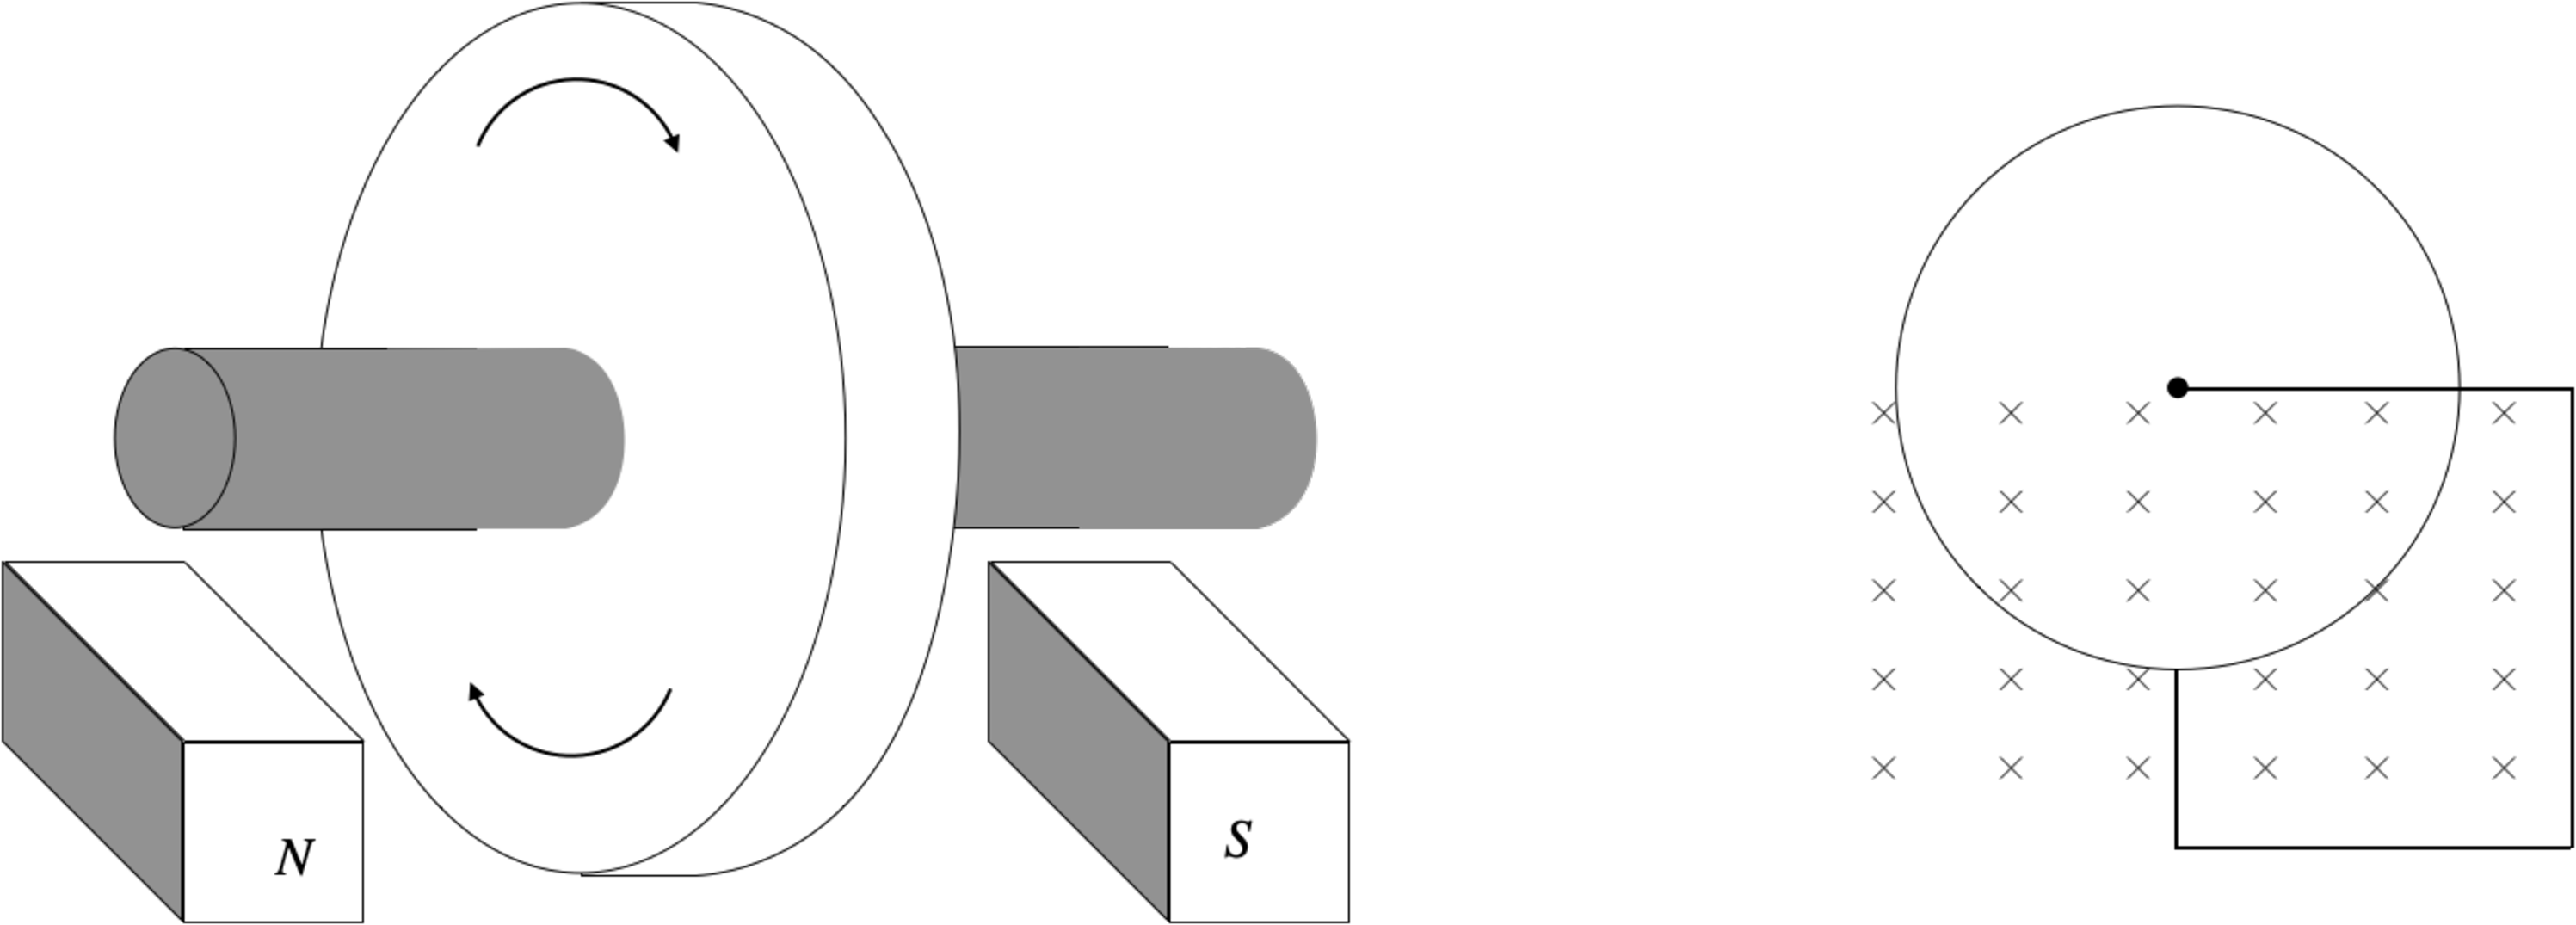
\includegraphics[width=5in]{figures/4.pdf} 
\end{center}	
\begin{itemize}
   \item the magnitude of induced e.m.f. is given by Faraday's law
      \[
      |E| = \left| - \frac{d\Phi}{dt}\right| = B \frac{dA}{dt} = B \frac{\pi r^2}{T} = BAf = \frac{1}{2}Br^2 \omega
      \]
      
\end{itemize}	

\section{Rotating coil in uniform magnetic field}
\begin{center}
   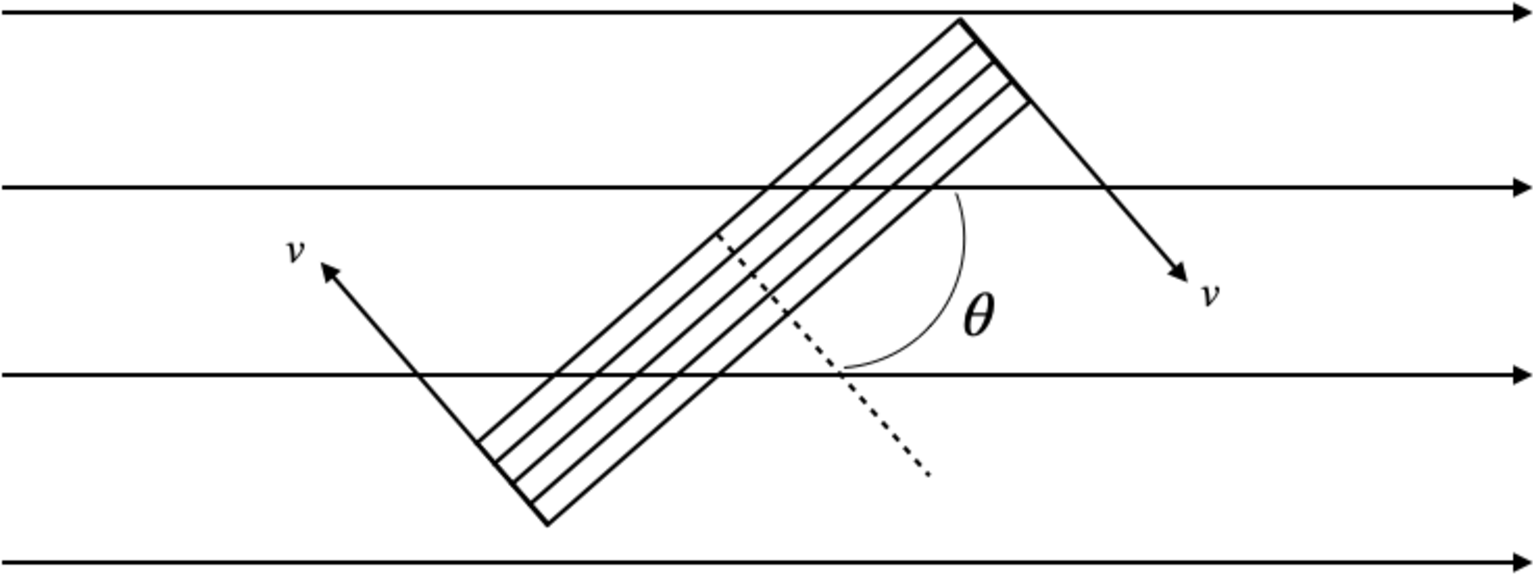
\includegraphics[width=3in]{figures/5.pdf} 
\end{center}	
\begin{itemize}
   \item the magnetic flux linkage is given by
      \[
      \Phi = NBA cos\theta = NBA cos \omega t
      \]
   \item By Faraday's law
     \begin{align*}
        E &= - \frac{d\Phi}{dt} \\ \\
          &= - \frac{d(NBAcos\omega t)}{dt} \\ \\
          &= -NBA \frac{d cos\omega t}{dt} \\ \\
          &= NBA \omega sin \omega t
     \end{align*}	 
      
\end{itemize}	


\end{document}	
